\subsection{YuvKA.Pipeline.PipelineDriver}

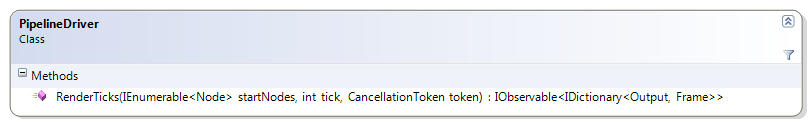
\includegraphics[width=\textwidth]{YuvKA.Pipeline/driver.png}
\begin{verbatim}
public class PipelineDriver
\end{verbatim}

\paragraph{Beschreibung}~\\
Die Klasse \name{PipelineDriver} ist für die Ausführung der Pipeline zuständig. Sie löst die gegenseitigen Abhängigkeiten der \name{Node}-Instanzen auf, um dann in Reihenfolge einer topologischer Sortierung deren \name{Process}-Methoden aufrufen zu können.
Die Klasse soll möglichst parallel implementiert werden, sodass mehrere aufeinanderfolgende Ticks gleichzeitig berechnet werden.

\paragraph{Typmember}
\begin{itemize}

\property{RenderTicks}
	\begin{verbatim}
public IObservable<IDictionary<Node.Output, Frame>> RenderTicks(
    IEnumerable<Node> startNodes, int tick, CancellationToken token)
    \end{verbatim}
	Berechnet die Pipeline ab dem angegebenen Tick und liefert eine asynchrone Aufzählung zurück, die pro Tick ein Dictionary enthält, das jedem Ausgang der gegebenen Knoten \name{startNodes} den jeweils berechneten Frame zuordnet.

    Parallelitätszusicherungen: Die Methode führt auf einer \name{Node}-Instanz \name{Process} immer seriell mit strikt aufsteigendem Tick aus. Die gleiche Ordnung gilt für den Rückgabewert. Die Berechnung wird bei Aktivierung des \name{token}s am nächstmöglichen Punkt beendet und beim nächsten Aufruf von \name{RenderTicks} erst gestartet, wenn alle vorhergehenden Berechungen beendet sind.

\end{itemize}
